\begin{figure}[h]
    \centering
    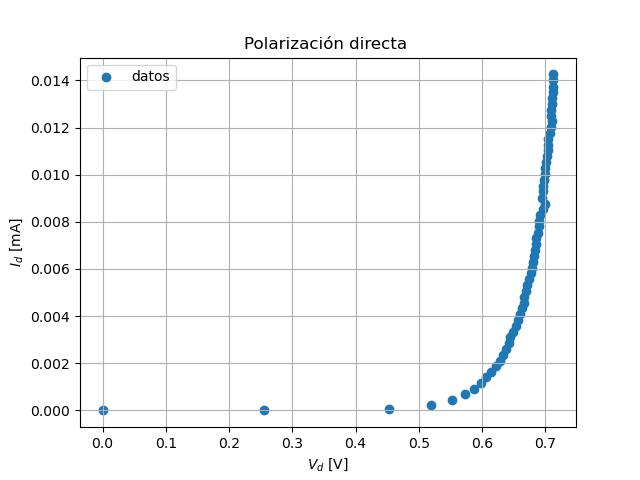
\includegraphics[width=\columnwidth]{figuras/pd_limpio.jpg}
    \caption{Corriente sobre diodo en polarizacion directa, variando el voltaje de $0 V$ a $15V$ en pasos de $0.5 V$, a una temperatura de $24 C^o$.}
    \label{pdlimpio}
\end{figure}


\begin{figure}[h]
    \centering
    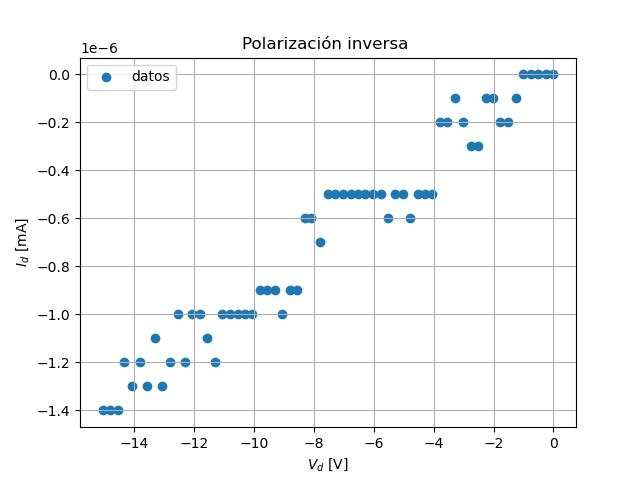
\includegraphics[width=\columnwidth]{figuras/pi_limpio.jpg}
    \caption{Corriente sobre diodo en polarizacion inversa, variando el voltaje de $0 V$ a $15V$ en pasos de $0.5 V$, a una temperatura de $24 C^o$.}
    \label{pilimpio}
\end{figure}

Para el ajuste lineal \textbf{insertar referencia} de la forma $y=mx+b$ donde $m=\beta /nT$ y $\beta = e/k_B$, con valores para este experimento $n=2$, $T=297.15 K$; se obtuvieron los siguientes resultados

\begin{table}
    \centering
    \begin{tabular}{ccc}
        $m=$ & $21.1 \pm 0.1 $ & $1/V$\\
        $b=$ & -$19.37 \pm 0.07$ &\\
        $R^2=$ & $0.998$ &\\
        $e/k_B =$ & $1.2528\times 10^4 \pm 64$ & $K/V$\\
        $E_{\%} =$ & $(7.96 \pm 0.55)\%$ &
    \end{tabular}
\end{table}


\begin{figure}[h]
    \centering
    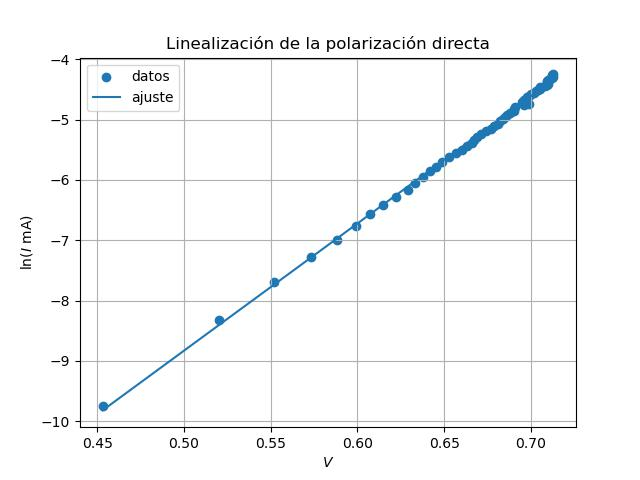
\includegraphics[width=\columnwidth]{figuras/pd_ajuste.jpg}
    \caption{Ajuste de la linealizacion \textbf{insertar referencia} para los datos obtenidos de la Figura \ref{pdlimpio}.}
    \label{pdajuste}
\end{figure}